\subsection{Starting a document}


% \begin{frame}[c,plain,noframenumbering]
% \begin{tikzpicture}[remember picture,overlay]
% \fill[fill=kul-blue]
%     (current page.south east)  rectangle  ([shift={(0,-0.1\paperheight)}]current page.north west)   ;
% \end{tikzpicture}

% \centering
% \vfill
% \textcolor{white}{\Large\textbf{Starting a document}}
% \end{frame}



\begin{frame}[fragile]{Starting a document}
Document class
\vspace{.5cm}
	\begin{columns}[t]
\begin{column}{.5\textwidth}
 \begin{minted}{latex}
    \documentclass{article}
    \begin{document}
        Hello world!
    \end{document}
 \end{minted}
\end{column}
		\begin{column}{.5\textwidth}
			\commo{documentclass} tells \latex\ how to lay out your document
			\vskip.05\textheight Standard classes are \Emph{article}, \Emph{report}, \Emph{book}, \Emph{letter}, \Emph{beamer} for presentations
			\vskip.05\textheight Each major publisher typically has its own class (e.g., IEEEtran)
		\end{column}
	\end{columns}	
\end{frame}

\begin{frame}[fragile]{Starting a document}
Preamble
\vspace{.5cm}
	\begin{columns}[t]
		\begin{column}{.5\textwidth}
			\texttt{\textcolor{blue}{\textbackslash documentclass}\textcolor{red}{\{}article\textcolor{red}{\}}
			\vskip.02\textheight
			
\begin{tikzpicture}
			\filldraw [fill=orange!30, draw=orange] (5.5,1) rectangle (0,0);
			\end{tikzpicture}
			\\\textcolor{olive}{\textbackslash begin\{document\}}
			\\\quad Hello world!
			\\\textcolor{olive}{\textbackslash end\{document\}}
			}
		\end{column}
		\begin{column}{.5\textwidth}
			In the \textcolor{orange}{preamble}, you define which packages to use
			\begin{itemize}
				\item \packopt{babel}{english}
				\item \pack{graphicx}
			\end{itemize}
			\somespace
                \packopt{graphicx}{option1, option2}
            
		\end{column}
	\end{columns}	
\end{frame}


\begin{frame}[fragile]{Starting a document}
Document itself
\vspace{.5cm}
	\begin{columns}[t]
		\begin{column}{.5\textwidth}
			\texttt{\textcolor{blue}{\textbackslash documentclass}\textcolor{red}{\{}article\textcolor{red}{\}}
			\vskip.1\textheight
			\textcolor{olive}{\textbackslash begin\{document\}}
			\\\quad Hello world!
			\\\textcolor{olive}{\textbackslash end\{document\}}
			}
		\end{column}
		\begin{column}{.5\textwidth}
			\textcolor{olive}{\textbackslash begin\{...\}} and \textcolor{olive}{\textbackslash end\{...\}} define\\ the beginning and the ending\\ of an \textit{environment}
			\vskip.05\textheight \textcolor{olive}{\textbackslash begin\{document\}} and \textcolor{olive}{\textbackslash end\{document\}} identify where your document\\ starts and stops
		\end{column}
	\end{columns}	
\end{frame}


% \begin{frame}[fragile,c]{Goal of today}
% \textbf{Show you the basics}
% \begin{itemize}
% 	\item Starting a document
% 	\item Text structuring
% 	\item Figures, Tables, Equations, Algorithms and Listings
% 	\item Bibliography
% \end{itemize}	
% \vskip.05\textheight
% What if you need more than the basics?
% \vskip.05\textheight
% Try it yourself!
% \end{frame}


% \begin{frame}[c,plain,noframenumbering]
% \begin{tikzpicture}[remember picture,overlay]
% \fill[fill=kul-blue]
%     (current page.south east)  rectangle  ([shift={(0,-0.1\paperheight)}]current page.north west)   ;
% \end{tikzpicture}
% \centering
% \vfill
% \textcolor{white}{\Large\textbf{Text structuring}}
% \end{frame}


\begin{frame}[fragile]{Including a Title and an Author}
\vspace{.5cm}
	\begin{columns}[t]
		\begin{column}{.5\textwidth}
			\texttt{\textcolor{blue}{\textbackslash documentclass}\textcolor{red}{\{}article\textcolor{red}{\}}
			\\\comm{title}{My First Document}
			\\\comm{author}{E. Peschiera}
			\\\comm{date}{}
			\\\textcolor{olive}{\textbackslash begin\{document\}}
			\\\quad\commo{maketitle}
			\\\quad Hello world!
			\\\textcolor{olive}{\textbackslash end\{document\}}
			}
		\end{column}
		\begin{column}{.5\textwidth}
			\comm{title}{...} and \comm{author}{...} \\are self-explanatory
			\vskip.05\textheight \comm{date}{} is useful to suppress the\\ showing of the current date
			\vskip.05\textheight \commo{maketitle} is fundamental! Without it,\\ title and author are excluded
		\end{column}
	\end{columns}	
    \somespace
    \somespace
    \begin{center}
        \Emph{Note: templates can define their own title/author commands.}
    \end{center}
\end{frame}

\begin{frame}[fragile]{Including a Title and an Author}
Result
\vspace{.5cm}
	\begin{columns}[t]
		\begin{column}{.5\textwidth}
			\texttt{\textcolor{blue}{\textbackslash documentclass}\textcolor{red}{\{}article\textcolor{red}{\}}
			\\\comm{title}{My First Document}
			\\\comm{author}{G. Callebaut}
			\\\comm{date}{}
			\\\textcolor{olive}{\textbackslash begin\{document\}}
			\\\quad\commo{maketitle}
			\\\quad Hello world!
			\\\textcolor{olive}{\textbackslash end\{document\}}
			}
		\end{column}
		\begin{column}{.5\textwidth}
			\begin{figure}
			
\includegraphics[width=.9\linewidth, frame, trim={-1cm -1cm -1cm -1cm},clip]{Figures/doc1}
			\end{figure}
		\end{column}
	\end{columns}	
\end{frame}

\begin{frame}[fragile]{Including Structuring Elements}
\vspace{.5cm}
	\begin{columns}[t]
		\begin{column}{.5\textwidth}
			Numbered elements
			\begin{itemize}
				\item \comm{chapter}{...}
				\item \comm{section}{...}
				\item \comm{subsection}{...}
				\item \comm{subsubsection}{...}
			\end{itemize}
			Unnumbered elements, same commands \\but with *
			\begin{itemize}
				\item \comm{chapter\textsuperscript{\textcolor{black}{*}}}{...}
			\end{itemize}
		\end{column}
		\begin{column}{.5\textwidth}
			Depending on the template, certain elements might not be present
			\begin{itemize}
				\item \comm{chapter}{} only in books and reports
				\item No structuring elements\\ supported in letters
			\end{itemize}
		\end{column}
	\end{columns}	
\end{frame}

\begin{frame}[fragile]{Including Structuring Elements}
%\vspace{.5cm}
	\begin{columns}[t]
		\begin{column}{.5\textwidth}
			\begin{figure}
			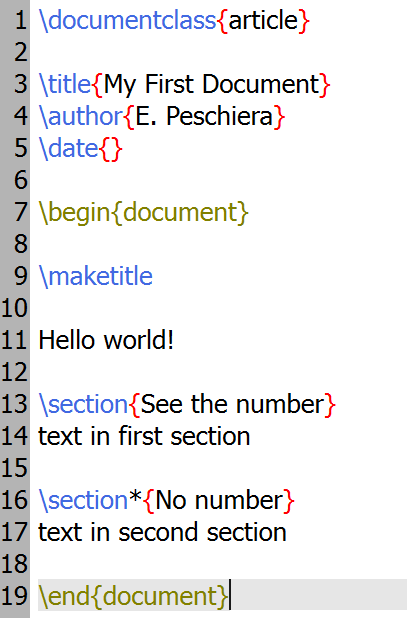
\includegraphics[scale=.5]{Figures/code1}
			\end{figure}
		\end{column}
		\begin{column}{.5\textwidth}
			\begin{figure}
			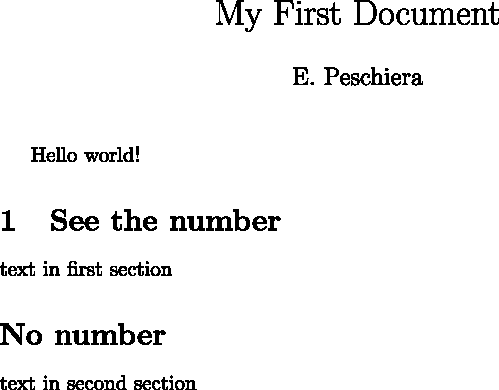
\includegraphics[width=.79\linewidth, frame, trim={-1cm -1cm -1cm -1cm},clip]{Figures/doc2}
			\end{figure}
		\end{column}
	\end{columns}	
\end{frame}
